\chapter{Manual de utilização} \label{manual}

Para usar o sistema desenvolvido, terá de executar os seguintes passos dentro da pasta Install:

\begin{enumerate}
	\item Dentro da pasta Storages existem três pastas. Em cada uma delas deverá lançar o executável \textit{KVStorage.exe};
	\item Dentro da pasta Brokers, existem duas pastas. Em cada uma delas, deverá lançar o executável \textit{Broker.exe};
	\item Para executar um ou mais clientes em .NET, deverá lançar o executável \textit{UserApp.exe} presente na pasta UserApps na sub-pasta dotNet;
	\item Para executar um ou mais clientes em Java, deverá ter instalado o Java e deverá lançar o .jar \textit{AppUser.jar} na linha de comandos com o comando "" presente na pasta UserApps na sub-paste java.
\end{enumerate}

\section{Utilização do Cliente}

\begin{figure}[h]
	\makebox[\textwidth][c]{
		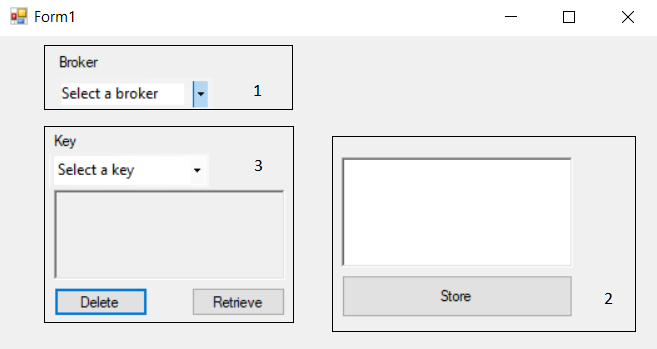
\includegraphics[width=0.9\textwidth]{./figures/userform}
	}
	\caption{User Form}
	\label{form}
\end{figure}

Na figura \ref{form} é apresentada a interface gráfica do utilizador.
Relativamente a esta figura, existem retângulos numerados. Cada retângulo é explicado de seguida.\\

No retângulo 1, pode selecionar o \textit{broker} à qual o utilizador pretende-se conectar.\\

No retângulo 2, é possível escrever um valor para ser guardado e pressionando o botão \textit{Store} irá comunicar com o \textit{broker} selecionado para tentar guardar o valor.\\

No retângulo 3, pode selecionar uma chave e estando a chave selecionado pode pedir o valor associado a essa chave clicando no botão \textit{Retrieve}. Ou então, pode eliminar o valor associado a essa chave clicando no botão \textit{Delete}.